% =========================================================================
% PHẦN TRÊN: LÝ THUYẾT & ĐỊNH NGHĨA 7 (BỐ CỤC 2 CỘT)
% =========================================================================

\noindent
\begin{minipage}[t]{0.26\textwidth}
  \vspace{0pt}
  \centering
  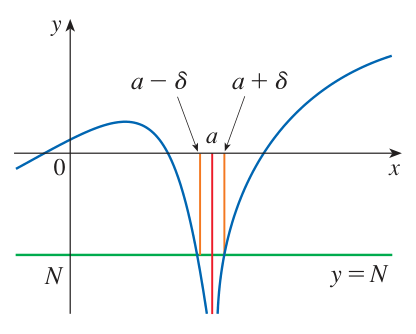
\includegraphics[width=\linewidth, keepaspectratio]{images/p0148_fig1.png}
  \vspace{3pt}
  
  {\small\textbf{\textsf{HÌNH 11}}}
\end{minipage}%
\hfill
\begin{minipage}[t]{0.71\textwidth}
  \vspace{0pt}
  Tương tự, dưới đây là phiên bản chính xác của Định nghĩa 2.2.5. Định nghĩa này được minh họa bởi Hình 11.

  \vspace{4pt}
  \begin{tcolorbox}[
    enhanced,
    colback=white,
    colframe=stewartred,
    boxrule=0.8pt,
    arc=0mm,
    top=5pt,
    bottom=5pt,
    left=8pt,
    right=8pt
  ]
    \setlength{\abovedisplayskip}{3pt}
    \setlength{\belowdisplayskip}{3pt}
    \noindent
    {\color{stewartred}\setlength{\fboxsep}{2pt}\setlength{\fboxrule}{0.8pt}\fbox{\bfseries 7}}\; 
    \textbf{\color{stewartred}\textsf{Định nghĩa}}\quad 
    Cho $f$ là một hàm số xác định trên một khoảng mở nào đó chứa số $a$, có thể ngoại trừ tại chính $a$. Khi đó
    \[
      \lim_{x \to a} f(x) = -\infty
    \]
    có nghĩa là với mọi số âm $N$ đều tồn tại một số dương $\delta$ sao cho
    \[
      \text{nếu} \quad 0 < |x - a| < \delta \quad \text{thì} \quad f(x) < N
    \]
  \end{tcolorbox}
\end{minipage}

\vspace{8pt}

% =========================================================================
% THANH TIÊU ĐỀ: 2.4 BÀI TẬP (3 ĐƯỜNG KẺ CYAN ĐẶC TRƯNG)
% =========================================================================

\noindent
\begin{tikzpicture}[x=1cm, y=1cm, baseline=(title.base)]
  % 3 vạch kẻ cyan trước tiêu đề
  \draw[stewartcyan, line width=0.6pt] (0, 0.16) -- (1.1, 0.16);
  \draw[stewartcyan, line width=0.6pt] (0, 0.08) -- (1.1, 0.08);
  \draw[stewartcyan, line width=0.6pt] (0, 0.00) -- (1.1, 0.00);

  % Tiêu đề
  \node[anchor=west, inner sep=0pt] (title) at (1.25, 0.08) {%
    {\fontsize{16}{19}\selectfont\bfseries\textsf{\color{stewartcyan}2.4}}\quad
    {\fontsize{14}{17}\selectfont\bfseries\textsf{Bài tập}}%
  };

  % 3 vạch kẻ cyan kéo dài đến lề phải
  \draw[stewartcyan, line width=0.6pt] (4.2, 0.16) -- (\linewidth, 0.16);
  \draw[stewartcyan, line width=0.6pt] (4.2, 0.08) -- (\linewidth, 0.08);
  \draw[stewartcyan, line width=0.6pt] (4.2, 0.00) -- (\linewidth, 0.00);
\end{tikzpicture}

\vspace{6pt}

% =========================================================================
% BÀI TẬP (CHIA 2 CỘT CÂN ĐỐI, VỪA KHÍT TRANG 1)
% =========================================================================

\noindent
\begin{minipage}[t]{0.48\textwidth}
  \vspace{0pt}
  \setlength{\parskip}{0pt}

  % BÀI TẬP 1
  \textbf{1.} Sử dụng đồ thị đã cho của hàm số $f$ để tìm một số $\delta$ sao cho
  \smallskip
  {\centering nếu\quad $|x - 1| < \delta$\quad thì\quad $|f(x) - 1| < 0.2$\par}
  \smallskip
  {\centering 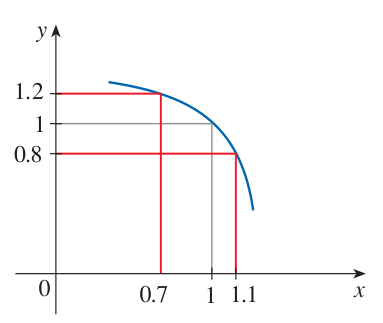
\includegraphics[height=2.5cm, keepaspectratio]{images/p0148_fig2.png}\par}

  \vspace{7pt}

  % BÀI TẬP 2
  \textbf{2.} Sử dụng đồ thị đã cho của hàm số $f$ để tìm một số $\delta$ sao cho
  \smallskip
  {\centering nếu\quad $0 < |x - 3| < \delta$\quad thì\quad $|f(x) - 2| < 0.5$\par}
  \smallskip
  {\centering 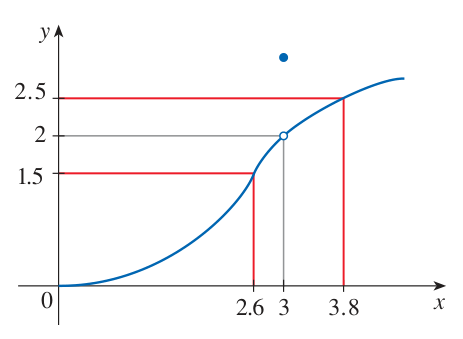
\includegraphics[height=2.6cm, keepaspectratio]{images/p0148_fig4.png}\par}

  \vspace{7pt}

  % BÀI TẬP 3
  \textbf{3.} Sử dụng đồ thị đã cho của hàm số $f(x) = \sqrt{x}$ để tìm một số $\delta$ sao cho
  \smallskip
  {\centering nếu\quad $|x - 4| < \delta$\quad thì\quad $|\sqrt{x} - 2| < 0.4$\par}
  \smallskip
  {\centering 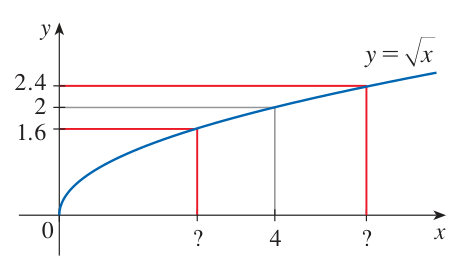
\includegraphics[height=2.4cm, keepaspectratio]{images/p0148_fig5.png}\par}
\end{minipage}%
\hfill
\begin{minipage}[t]{0.485\textwidth}
  \vspace{0pt}
  \setlength{\parskip}{0pt}
  \setlength{\abovedisplayskip}{3pt}
  \setlength{\belowdisplayskip}{3pt}

  % BÀI TẬP 4
  \textbf{4.} Sử dụng đồ thị đã cho của hàm số $f(x) = x^2$ để tìm một số $\delta$ sao cho
  \smallskip
  {\centering nếu\quad $|x - 1| < \delta$\quad thì\quad $|x^2 - 1| < \tfrac{1}{2}$\par}
  \smallskip
  {\centering 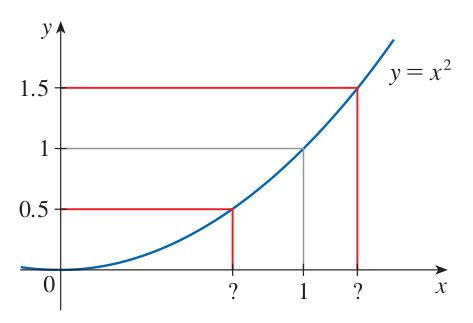
\includegraphics[height=2.5cm, keepaspectratio]{images/p0148_fig3.png}\par}

  \vspace{5pt}

  % BÀI TẬP 5
  \noindent\graphicon\ \textbf{5.} Sử dụng đồ thị để tìm một số $\delta$ sao cho
  \smallskip
  {\centering nếu\quad $|x - 2| < \delta$\quad thì\quad $|\sqrt{x^2 + 5} - 3| < 0.3$\par}

  \vspace{5pt}

  % BÀI TẬP 6
  \noindent\graphicon\ \textbf{6.} Sử dụng đồ thị để tìm một số $\delta$ sao cho
  \smallskip
  {\centering nếu\quad $\left|x - \dfrac{\pi}{6}\right| < \delta$\quad thì\quad $\left|\cos^2 x - \dfrac{3}{4}\right| < 0.1$\par}

  \vspace{5pt}

  % BÀI TẬP 7
  \noindent\graphicon\ \textbf{7.} Đối với giới hạn
  \[
    \lim_{x \to 2} (x^3 - 3x + 4) = 6
  \]
  hãy minh họa Định nghĩa 2 bằng cách tìm các giá trị của $\delta$ tương ứng với $\varepsilon = 0.2$ và $\varepsilon = 0.1$.

  \vspace{5pt}

  % BÀI TẬP 8
  \noindent\graphicon\ \textbf{8.} Đối với giới hạn
  \[
    \lim_{x \to 0} \frac{e^{2x} - 1}{x} = 2
  \]
  hãy minh họa Định nghĩa 2 bằng cách tìm các giá trị của $\delta$ tương ứng với $\varepsilon = 0.5$ và $\varepsilon = 0.1$.

  \vspace{5pt}

  % BÀI TẬP 9
  \noindent\graphicon\ \textbf{9.} (a) Sử dụng đồ thị để tìm một số $\delta$ sao cho
  \smallskip
  {\centering nếu\quad $2 < x < 2 + \delta$\quad thì\quad $\dfrac{1}{\ln(x - 1)} > 100$\par}
  \smallskip
  \noindent\hspace*{1.3em}(b) Phần (a) gợi ý giới hạn nào là đúng?
\end{minipage}
